\section{Mathematical Models of the Heart}

Cardiac tissue has been modelled mathematically for about fifty years.
While initial models were simple, there are now models of high sophistication
available.
These models are capable of reproducing both healthy and pathological behaviour
with some accuracy.

\subsection{Categorising Myocyte Models}

Cellular models tend to be classified in two ways.
The first differentiator is the level of detail employed.
The second is on which cellular processes are modelled.

Biophysically detailed models are complex.
They consider the interactions of several different currents, and potentially
intra- and extracellular ion concentrations, reservoirs as well as other
details.
The second type are simplified, phenomenological, models.
These do not consider individual ion concentrations but instead just reproduce
one desired factor, typically the action potential profile.

Models, whether biophysically detailed or not, can concern themselves with the
cellular electrophysiology, the mechanical contractions or both.
This thesis concerns itself just with electrophysiological models.
Models of the mechanics are not considered and are not treated in this
description of mathematical modelling.

\subsection{A Brief History of Cardiac Myocyte Modeling}

The first model of cardiac electrophysiology was published by
Noble~\cite{Noble1962}, and modelled Purkinje fibre (A specialised part of the
ventricular conduction system) action potentials.
Shortly thereafter, various refinements were published, as further experimental
data became available.
This was eventually followed by the Beeler--Reuter~\cite{Beeler1977}\ model of
the guinea pig ventricular myocyte.

The Luo--Rudy guinea pig ventricular myocyte model was first published in
1991~\cite{Luo1991} and was then sub-sequentially majorly revised and
republished in 1994~\cite{Luo1994}.
The first Luo-Rudy model was based on the Beeler--Reuter model, though with updated channel behaviours
and more complex potassium channels.
The second Luo-Rudy model was the first of the `second generation' models,
with fluctuations in all ion concentrations, and a much more detailed series of
equations for calcium handling.

In 1998, the Courtemanche--Ramirez--Natel\cite{CRN98}\ (CRN) model and the
Nygren~\cite{Nygren1998}\ model were published.
These were both models of the human atrium.
They were also both second generation models, with detailed calcium handling.
Also in 1998 Fenton and Karma published their phenomenological
Fenton--Karma~\cite{Fenton1998}\ model, which used just three channels to
reproduce the shape of the ventricular action potential.

\subsection{Mathematical Models of Myocytes}

Mathematical models of cardiac myocytes are built from a few simple assumptions
and considerations.
These concern the behaviour of the cellular membrane and ion channels.
The important ones are detailed here.

\subsubsection{The Nernst Equilibrium Potential}

The Nernst equation is an important equation in electrophysiology~\cite{Fall2002}.
It describes how the difference in ion concentrations on two sides of a
semi-permeable barrier can result in a potential difference across the barrier.
Any voltage dependant factor of a current of an ion, S, includes a reversal
potential, V$_{S}$, equal to the Nernst potential.
At the reversal potential, the current falls to 0.
When equilibrium is reached the potential difference, $V_{S}$, across the
membrane is given by
\begin{equation}
V_{S} = \frac{RT}{zF}ln\left( \frac{[S]_{e}}{[S]_{i}} \right) 
\end{equation} 
where subscripts $i$ and $e$ denote internal and external concentrations of S,
$R$ is the universal gas constant, $T$ is the absolute temperature, $F$ is
Faraday's constant and $z$ the charge of the ion $S$.

The Nerst Potential applies only to a single ion concentration.
This is not as large a limitation as it first might seem.
Whilst the action potential involves many ion species, many channels are ion
specific and thus the Nerst potential applies across them.

\subsubsection{Electric Circuit Model}

\begin{figure}
\begin{center}
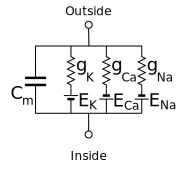
\includegraphics{figures/intro/electrical_circuit_cell}
\end{center}
\caption[Electrical Circuit Model Of The Cell]{
\label{fig:intro:math:circuit}
Electrical circuit representation of the cell.
The cell membrane is represented by a capacitance, $\text{C}_{\text{m}}$.
There are three currents, represented by the resistances $\text{g}_{\text{K}}$, 
$\text{g}_{\text{Ca}}$ and $\text{g}_{\text{Na}}$.
The current through the resistances is driven by the three Nernst potentials,
$\text{E}_{\text{K}}$, 
$\text{E}_{\text{Ca}}$ and $\text{E}_{\text{Na}}$.
}
\end{figure}

The electrical circuit model of the cell membrane underpins much of the work in
modelling the behaviour of cardiac myocytes.
It is however a very simple concept.
Since the membrane separates charges, it may be considered as a capacitor, as
shown in figure~\ref{fig:intro:math:circuit}.
Since there is no net buildup of
charge on either side of the membrane, any ionic current, \ii{ion}, must be
countered by a capacitive current, and so
\begin{equation}
C_{m}\frac{dV_{m}}{dt} + \ii{ion} = 0
\label{eqn:intro:math:basic}
\end{equation}
where $V_{m}$ is the membrane voltage, and is defined as the difference between
the internal potential, $u_{i}$ and the external potential, $u_{e}$ or
\begin{equation}
V_{m} = u_{i} - u_{e}
\label{eqn:intro:math:vm}
\end{equation}
When multiple currents are considered, the total inward and outward currents are
summed.
The difficulty comes in determining the form of \ii{ion}, which varies widely
depending on the nature of the channel or pump in question.


\subsubsection{The Hodgkin-Huxley Equations}

Many mathematical models of cardiac myocytes feature one or more
`Hodgkin--Huxley' channels.
Hodgkin and Huxley developed them in a now classic series of papers concerning
the current flow through the membrane of the squid giant
axon~\cite{Hodgkin1952,Keener1998}.
They characterise the current flow with elegance and surprising accuracy.
It is important to note that the Hodgkin--Huxley equations consider the bulk
behaviour of the many thousands of individual channel structures distributed
across the membrane, not the behaviour of one single channel.

Hodgkin and Huxley started with a very simple assumption.
The current flow through a channel on the membrane, $I_{S}$ is given by
\begin{equation}
I_{S} = g_{S}\left(V-V_{S}\right)
\label{eqn:intro:math:hh1}
\end{equation}
where $g_{S}$ is the channel conductance, $V$ the membrane potential and $V_{S}$
the Nernst potential for the ion $S$.
Equation (\ref{eqn:intro:math:hh1}) assumes that the channel is selective for
one ion species S, and that the current is a simple linear function of the
voltage across the membrane.

With this underlying assumption, Hodgkin and Huxley set out to accurately map
the behaviour of the current with regards time and voltage.
The following section explains the description for the sodium current, \ii{Na}.
From the form of the sodium channel under voltage clamp conditions, it is
reasonable to expect $g_{Na}$ obeys a differential equation of the form
\begin{equation}
\frac{dg_{Na}}{dt} = f\left(v,t\right)
\label{eqn:intro:math:hh2}
\end{equation}
where $v=V-V_{Na}$.
However, the form of $g_{Na}$ is complex.
While remaining at the same voltage, the conductance at first increases and then
tails off.
It appeared that there were two processes at work, one that turned the current
on, and one that turned it off.
Hodgkin and Huxley realised that it would be easier to write $g_{Na}$ as a
function of two different variables.
One which corresponded to the turning on and one to the turning off of the
channel.
This leads there being an activation variable, called $m$, an inactivation
variable, called $h$ and that the current would be some linear combination of the
two, multiplied by a constant conductance factor $\bar{g}_{Na}$.
The two variables $m$ and $h$ would both satisfy a differential equation such as
\begin{equation}
\frac{dm}{dt}=\alpha_{m}\left(v\right)\left(1-m\right) -
\beta_{m}\left(v\right)m
\label{eqn:intro:math:dmdt}
\end{equation}
where $\alpha_{m}$ and $\beta_{m}$ are functions of $v\,\left(=V-V_{Na}\right)$.
As an activation $m$, $\alpha_{m}$ and $\beta_{m}$ are such that $m$ is
initially small but increases with the potential.
As $h$ is an inactivation, $\alpha_{h}$ and $\beta_{h}$ give an initially high
value of $h$ that then decays, inactivating the channel.

The form proposed for $g_{Na}$ by Hodgkin and Huxley was
\begin{equation}
g_{Na}=\bar{g}_{Na}m^{3}h
\label{eqn:intro:math:gna}
\end{equation}
where all symbols are as defined previously.
The decision to raise $m$ to the third power was based on the rate of increase
observed in voltage clamp experiments.
It is interesting to note that when the structure of \ii{Na}\ was examined in
detail, it was discovered that the channel has three structures which open to
allow current to flow.
A second structure, the `ball and chain' then acts to close the channel.

Many different channels are modelled as Hodgkin--Huxley channels.
Different channels have different activation and inactivation variables.
These variables are modulated by different $\alpha$ and $\beta$ equations.

\subsubsection{Markov Chain Descriptions Of Ion Channels}

Markov chain models of ion channels~\cite{Balser1990,Clancy1999,Silva2005}\
emerged when more detailed information on ion channel behaviour became
available.
This included single channel recordings rather than whole cell recordings.
Under such conditions, as well as in certain pathological states, the
Hodgkin--Huxley descriptions of the cells broke down.

In a markov chain model, instead of having one or more activations or
inactivations, the channel has a number of states.
Common states can include open, inactive and closed.
A channel can have more than one state of each sort.
Transitions are only allowed between certain states and each transition has a,
usually time or voltage dependent, probability.
Channels only allow current to flow whilst in an open state.

Markov chain models can be highly complex and contain many states.
They can be utilised in a variety of ways.
One markov chain can represent the behaviour of all the individual channels on
the cell.
In this case, the total current flowing in the channel will be proportional to
the fraction of open states.
Cells can also have multiple markov chains to represent the flow through a
channel, each with its own proportions of state occupancy.
They also open the possibility of using stochastic simulation techniques where
the transition between states is controlled by random chance.

\subsection{Selected Myocyte Models}

There are tens, perhaps hundreds, of myocyte models of varying complexity and
accuracy.
There are relatively few models of atrial myocytes for human tissue.
A brief description of the foremost two are given here, as well as a description
of one of the most adaptable phenomological models.

\subsubsection{The Courtemanche--Rameriz--Nattel Model}

The Courtemanche--Rameriz--Nattel (CRN) model~\cite{CRN98}\ is a biophysically
detailed second generation model of the human atrial myocyte.
It was based on the Luo-Rudy~\cite{Luo1994}\ model of the guinea pig ventricular
myocyte.
The currents were then modified based on data from human and animal atrial
myocytes.

The CRN model tracks 21 state variables.
Most of these are gating parameters for the many ion channels, but the model
also tracks the internal concentration of potassium, sodium and calcium ions.
The external concentrations of ions are assumed constant.
There are also state parameters representing the calcium stored in internal
structures, such as the sarcoplasmic reticulum.
\begin{equation}
\label{eqn:intro:math:crn}
\ii{ion} = \ii{Na} + \ii{K1} + \ii{to} + \ii{Kur} + \ii{Kr} + \ii{Ks} +
\ii{Ca,L} + \ii{b,Na} + \ii{b,Ca} + \ii{NaK} + \ii{NaCa} + \ii{p,Ca}
\end{equation}
The CRN has 12 transmembrane currents which contribute to \ii{ion},
equation~(\ref{eqn:intro:math:crn}), and pumps and 4 currents and
pumps which just interact with the internal calcium stores.
The external currents are \ii{Na}, the fast sodium current, \ii{K1}, the inward
rectifier calcium current, \ii{to}, the transient outward current, \ii{Kur}, the
ultra-rapid delayed rectifier current, \ii{Kr}, the rapid delayed rectifier
current, \ii{Ks}, the slow delayed rectifier current, \ii{Ca,L}, the L-type
calcium current, \ii{b,Na}, the sodium background current and \ii{b,Ca}, the
calcium background current.
All the currents are time-dependent, except for the background currents which
have constant coductance and \ii{K1}, which is voltage-dependent.
There are also three pumps; \ii{NaK}, the sodium--potassium exchanger,
\ii{NaCa}, the sodium--calcium exchanger and \ii{p,Ca}, the calcium pump.

As a biophysically detailed model, the CRN model is suitable for a variety of
modeling tasks.
The number of currents make it an attractive option for modeling drugs or
genetic mutations.
It can be expensive to solve for large numbers of cells, however.

\subsubsection{The Nygren Model}

The Nygren model~\cite{Nygren1998}\ is a biophysically detailed second
generation model of the human atrial myocyte.
It was based on the Linblad~\cite{Lindblad1996} model of the rabbit atrium.
The equations were then modified using human data, mostly gathered from the
atrial appendages.

The Nygren model tracks 29 state variables.
Most of these are gating parameters.
They model also tracks concentrations of ions, both internally and in
extracellular cleft spaces, to represent local ion fluctuations.
Like the CRN model, there are also variables to represent internal calcium
handling.
\begin{equation}
\label{eqn:intro:math:nygren}
\ii{ion} = \ii{Na} + \ii{K1} + \ii{to} + \ii{Kur} + \ii{Kr} + \ii{Ks} +
\ii{Ca,L} + \ii{b,Na} + \ii{b,Ca} + \ii{NaK} + \ii{NaCa} + \ii{p,Ca}
\end{equation}
The Nygren model has 12 transmembrane currents which contribute to \ii{ion},
equation~(\ref{eqn:intro:math:nygren}), and pumps and 4 currents and
pumps which just interact with the internal calcium stores.
The external currents are \ii{Na}, the fast sodium current, \ii{K1}, the inward
rectifier calcium current, \ii{to}, the transient outward current, \ii{Kur}, the
ultra-rapid delayed rectifier current, \ii{Kr}, the rapid delayed rectifier
current, \ii{Ks}, the slow delayed rectifier current, \ii{Ca,L}, the L-type
calcium current, \ii{b,Na}, the sodium background current and \ii{b,Ca}, the
calcium background current.
All the currents are time-dependent, except for the background currents which
have constant coductance and \ii{K1}, which is voltage-dependent.
There are also three pumps; \ii{NaK}, the sodium--potassium exchanger,
\ii{NaCa}, the sodium--calcium exchanger and \ii{p,Ca}, the calcium pump.

The Nygren model is a biophysically detailed model, suitable for a variety of
modelling tasks.
It has more involved mathematics and requires more storage than the CRN model,
making it less attractive for large-scale simulation.
It is also interesting to note that the two models have very different
AP morphologies, the reasons for which have been the subject of some
research~\cite{Nygren2001,Syed2005,Cherry2008}.

\subsubsection{The Fenton--Karma Model}

The Fenton--Karma (FK) model~\cite{Fenton1998,Bueno-Orovio2008}\ is a
phenomenological, or minimal variable, model of the ventricular action
potential.
The goal of the FK model is to accurately reproduce the AP profile and
restitution properties of myocytes as well as short-term memory effects.
The original FK model has 3 variables, a fourth was added recently.

The FK model tracks 4 state variables.
These have no real physiological analogues.
\begin{equation}
\label{eqn:intro:math:fko}
\ii{ion} = \ii{fi} + \ii{si} + \ii{so}
\end{equation}
The FK model has 3 transmembrane currents which contribute to \ii{ion},
equation~(\ref{eqn:intro:math:fko}).
The fast inward current, \ii{fi}, is roughly analogous to the fast sodium
current in more detailed models, the slow inward current, \ii{si}, fulfils a
similar role to the L-type calcium current and the slow outward current, \ii{si},
is analogous to the potassium rectifier currents.
The behaviour of the currents is generally controlled by step functions based
on the state variables.

The FK model is not biophysically detailed.
This makes it very fast to solve, making it attractive for large tissue
simulations.
The drawback of this is that incorporating complex hormonal or drug interactions
is difficult.
The model is highly modifiable, with parameter sets that can reproduce a variety
of AP morphologies and restitution behaviours, including one for atrial myocyte
APs~\cite{Weber2008}.

\subsection{Models of Action Potential Propagation}

Single myocyte models are important, and can tell us much about the heart in
disease and health.
The heart is not made up of isolated myocytes however.
Whilst current computational power does not allow myocytes to be modelled on an
individual cellular basis for the whole heart, continuum models of propagation
have been developed.
These are summed up in the bidomain equations, and their simplification, the
monodomain equations.

\subsubsection{The Bidomain Equation}

The bidomain equation comes out of basic electromagnetic theory and several
assumptions about the nature of cardiac tissue~\cite{Tung1978,Geselowitz1983}.
\begin{enumerate}
    \item The cardiac tissue contains two continuous, simply connected domains, the intracellular and extracellular domains.
    There is no detailed consideration of the fine points of geometry.
    \item The intra- and extracellular domains overlap and fill all of the cardiac muscle. Each point lies in both domains.
    \item Charge does not accumulate.
\end{enumerate}

The derivation is not that difficult to work through, and it results in the bidomain equations
\begin{subequations}
\label{eqn:intro:math:bidom}
\begin{align}
\underline{\nabla}\cdot\left(\left(M_{i}+M_{e})\right)\underline{\nabla}u_{e}\right) + \underline{\nabla}\cdot\left( M_{i}\underline{\nabla}V_{m}\right) &=& 0
\label{eqn:intro:math:bidom1}\\
\underline{\nabla}\cdot\left(M_{i}\underline{\nabla}V_{m}\right) + \underline{\nabla}\cdot\left(M_{i}\underline{\nabla}u_{e}\right) &=& \chi C_{m}\frac{dV_{m}}{dt} + \chi{I_{ion}}
\label{eqn:intro:math:bidom2}
\end{align}
\end{subequations}
where the subscript $i$ and $e$ refer to the intra- and extracellular quantities, $M$ is a matrix of conductivities, $\chi$ represents the surface-to-volume ratio of the cells and all other quantities are as defined previously.
The bidomain equations are a coupled set of a parabolic and elliptic differential equation.

Boundary conditions for the bidomain equations vary, though the most common ones are described here.
First, no intracellular fluxes leave the heart.
Second, the body is assumed to be a passive conductor that is isolated at the outer surface.
The body potential at the surface of the heart is the extra-cellular potential at the surface of the heart.

\subsubsection{The Monodomain Equation}

While the bidomain equations represent a good tool for modelling some of the complexities of cardiac conduction, they are very demanding to solve, necessitating finding the solution to coupled parabolic and elliptic differential equation sets.
The monodomain equation is the result of one simplifying assumption made to the bidomain equations.
For the monodomain equation, we assume that the anisotropy ratio, $\lambda$, is the same for the intra- and extra-cellular fluids at all points.
\begin{equation}
M_{i} = {\lambda}M_{e}
\label{eqn:intro:math:mratio}
\end{equation}
This assumption is not a very physiological one, but the simplification it
allows is significant and so it is quite commonly used.

Substituting (\ref{eqn:intro:math:mratio}) into (\ref{eqn:intro:math:bidom1})
and (\ref{eqn:intro:math:bidom2}) and rearranging reduces the pair of equations
to one single equation for the membrane potential
\begin{equation}
\frac{\lambda}{1+\lambda}\underline{\nabla}\cdot\left(M_{i}\underline{\nabla}V_{m}\right) = \chi C_{m}\frac{dV_{m}}{dt} + \chi{I_{ion}}
\label{eqn:intro:math:mono}
\end{equation}
Typically, the factor of ${\lambda}/\left({1+\lambda}\right)$ is folded into $M_{i}$ to give the diffusion tensor $D$.
In 1D, this is the cable equation, which is very widely used.
The values of the components of the tensors $M_{i}$ or $D$ may be determined experimentally, or from a comparison of conduction in real and virtual tissue samples.

\subsection{Numerical Techniques}

There exist a wealth of techniques for solving the ordinary differential
equations (ODEs) and partial differential equations (PDEs) involved in
mathematical models~\cite{Sundnes2006}.
These techniques vary in complexity and accuracy.
The correct choice of technique depends on a number of factors including the
`stiffness' of the equations, the desired accuracy and others.

\subsubsection{The Forward Euler Method}

The forward Euler method~\cite{Birkhoff1989}\ is perhaps the simplest numerical
integration technique.
It requires a relatively small (time) step between integration points.
It is never--the--less quite suitable to use in simulations of the electrical
activity of the heart.
A typical set of ODEs representing the electrical activity of a myocyte are very
`stiff', which is to say they can be numerically unstable if the step size is
too large, and so more sophisticated methods can also require a very small
timestep.

The forward Euler method works as follows.
If we have a function, $f(t, u)$, for which we know the initial
values, $(t_0, u_0)$, then by assuming the rate of change of $f$ remains constant
over some small interval, $h$, we can integrate the equation as follows
\begin{subequations}
\label{eqn:intro:euler}
\begin{align}
t_{n+1} = & t_n + h \label{eqn:intro:euler:t} \\
u_{n+1} = & u_n + hf(t_n, u_n) \label{eqn:intro:euler:x}
\end{align}
\end{subequations}
As long as the interval is small enough the sequence $u_1,u_2,\cdots,u_n$
should be a good approximation of the time evolution of $u$.
If we have more than one value on the right hand side of the equation ($u =
u^{(1)}, u^{(1)}, \cdots, u^{(n)}$) then all values of the right hand side are
assumed constant for each step of the integration.
In cardiac systems, $h$ is typically \ms{0.02}\ or smaller.

\subsubsection{The Finite Difference Method}

The finite difference method~\cite{Morton2005} is a way of calculating the
solution to a spatially extended problem.
Such problems include PDEs such as the bidomain (\ref{eqn:intro:math:bidom}) and
monodomain (\ref{eqn:intro:math:mono}) equations.
The general form of such equations in the variable $u(t, u)$ is
\begin{equation}
\label{eqn:intro:fd:partial}
\frac{\partial u}{\partial t} = \frac{\partial}{\partial x} \left( b(t, x)
\frac{\partial u}{\partial x} \right) + c(t, x)u + d(t, x) + e(t, u)
\end{equation}
Where $t$ is the time, $x$ is the spatial variable and $b$, $c$, $d$ and $e$ are
known functions.
The function $e$ will quite often be \ii{ion}\ for a particular cell.

In the finite difference method, the problem space---the cardiac tissue, in this
thesis---is divided up into a number of nodes.
The spacing between each node is $\Delta x$ in the x direction (and in higher
dimensions,  $\Delta y$ in the y direction and so on).
To advance the solution in time, the forward Euler method
(\ref{eqn:intro:euler}) can be used.
To approximate the differential in space, the centred second difference can be
used.
For the node at $x_i$ at time $t_n$ it is:
\begin{equation}
\label{eqn:intro:fd:secondcentral}
\frac{\partial^2 u}{\partial x^2}\left(x_i, t_n\right) \approx \frac{u(x_{i+1},t_n) - 2u(x_{i},t_n) + u(x_{i-1},t_n) }{\left(\Delta x\right)^2}
\end{equation}
where $i$ is the index of the node, and $n$ the index of the instant of time.
The space centered first difference (needed when conductional anisotropy is to
be taken into account) is:
\begin{equation}
\label{eqn:intro:fd:firstcentral}
\frac{\partial u}{\partial x}\left(x_i, t_n\right) \approx \frac{u(x_{i+1},t_n) - u(x_{i-1},t_n) }{2\left(\Delta x\right)}
\end{equation}

The most common boundary conditions we want to apply are Neumann, `no flux',
boundary conditions where the differential of $u$ with respect to $x$ is set to
zero at the edges of the tissue.
At the edge of the tissue, the approximation for the space differential
(\ref{eqn:intro:fd:secondcentral}) becomes:
\begin{equation}
\label{eqn:intro:fd:secondcentralboundary}
\frac{\partial^2 u}{\partial x^2}\left(x_i, t_n\right) \approx \frac{2\left((u(x_{i-1},t_n) - u(x_{i},t_n) \right)  }{\left(\Delta x\right)^2}
\end{equation}
if the node at $x_{i+1}$ would be `outside' the tissue.
The approximation if the converse is true ($x_{i-1}$ is outside) replaces
$x_{i-1}$ with $x_{i+1}$.
The one dimensional approximation becomes:
\begin{equation}
\label{eqn:intro:fd:firstcentralboundary}
\frac{\partial u}{\partial x}\left(x_i, t_n\right) \approx \frac{u(x_{i},t_n) - u(x_{i-1},t_n) }{\left(\Delta x\right)}
\end{equation}
again, for if the node $x_{i+1}$ is outside.

In higher orders, (\ref{eqn:intro:fd:secondcentral}) and
(\ref{eqn:intro:fd:firstcentral}) are applied along each direction.
The nodes used in the calculation of the value $u_x$ are known as the stencil.
The typical 5-node stencil used for solving (\ref{eqn:intro:fd:partial}) and
hence (\ref{eqn:intro:math:bidom}) or (\ref{eqn:intro:math:mono}) is illustrated
in figure~\ref{fig:intro:math:stencil}.
Other schemes can use different stencils.


\subsubsection{The Rush--Larsen Technique}


